% !TEX root = ../main.tex
Для перевірки результатів леми \ref{main_lemma} та теорем
\ref{th:min_max_limit}, \ref{th:sum_limit}, \ref{th:spacing_limit}
скористаємося процесом китайського ресторану для отримання вибірок
з $\ESF{n, \theta}$. Розмір вибірки в усіх випадках буде рівний 3000.

\subsection{Розподіл кількості нерухомих точок}
Для демонстрації збіжності ймовірностей
$\P{X_n = k} \to \P{N = k}$, де $N \sim \Poiss{\theta}$,
а $X_n$ визначено в лемі \ref{main_lemma} при $\gamma = 1$,
порівняємо полігони розподілу для $X_n$ при $n = 50, 100, 500$ для
різних значень $\theta$.
\begin{figure}[H]
    \centering
    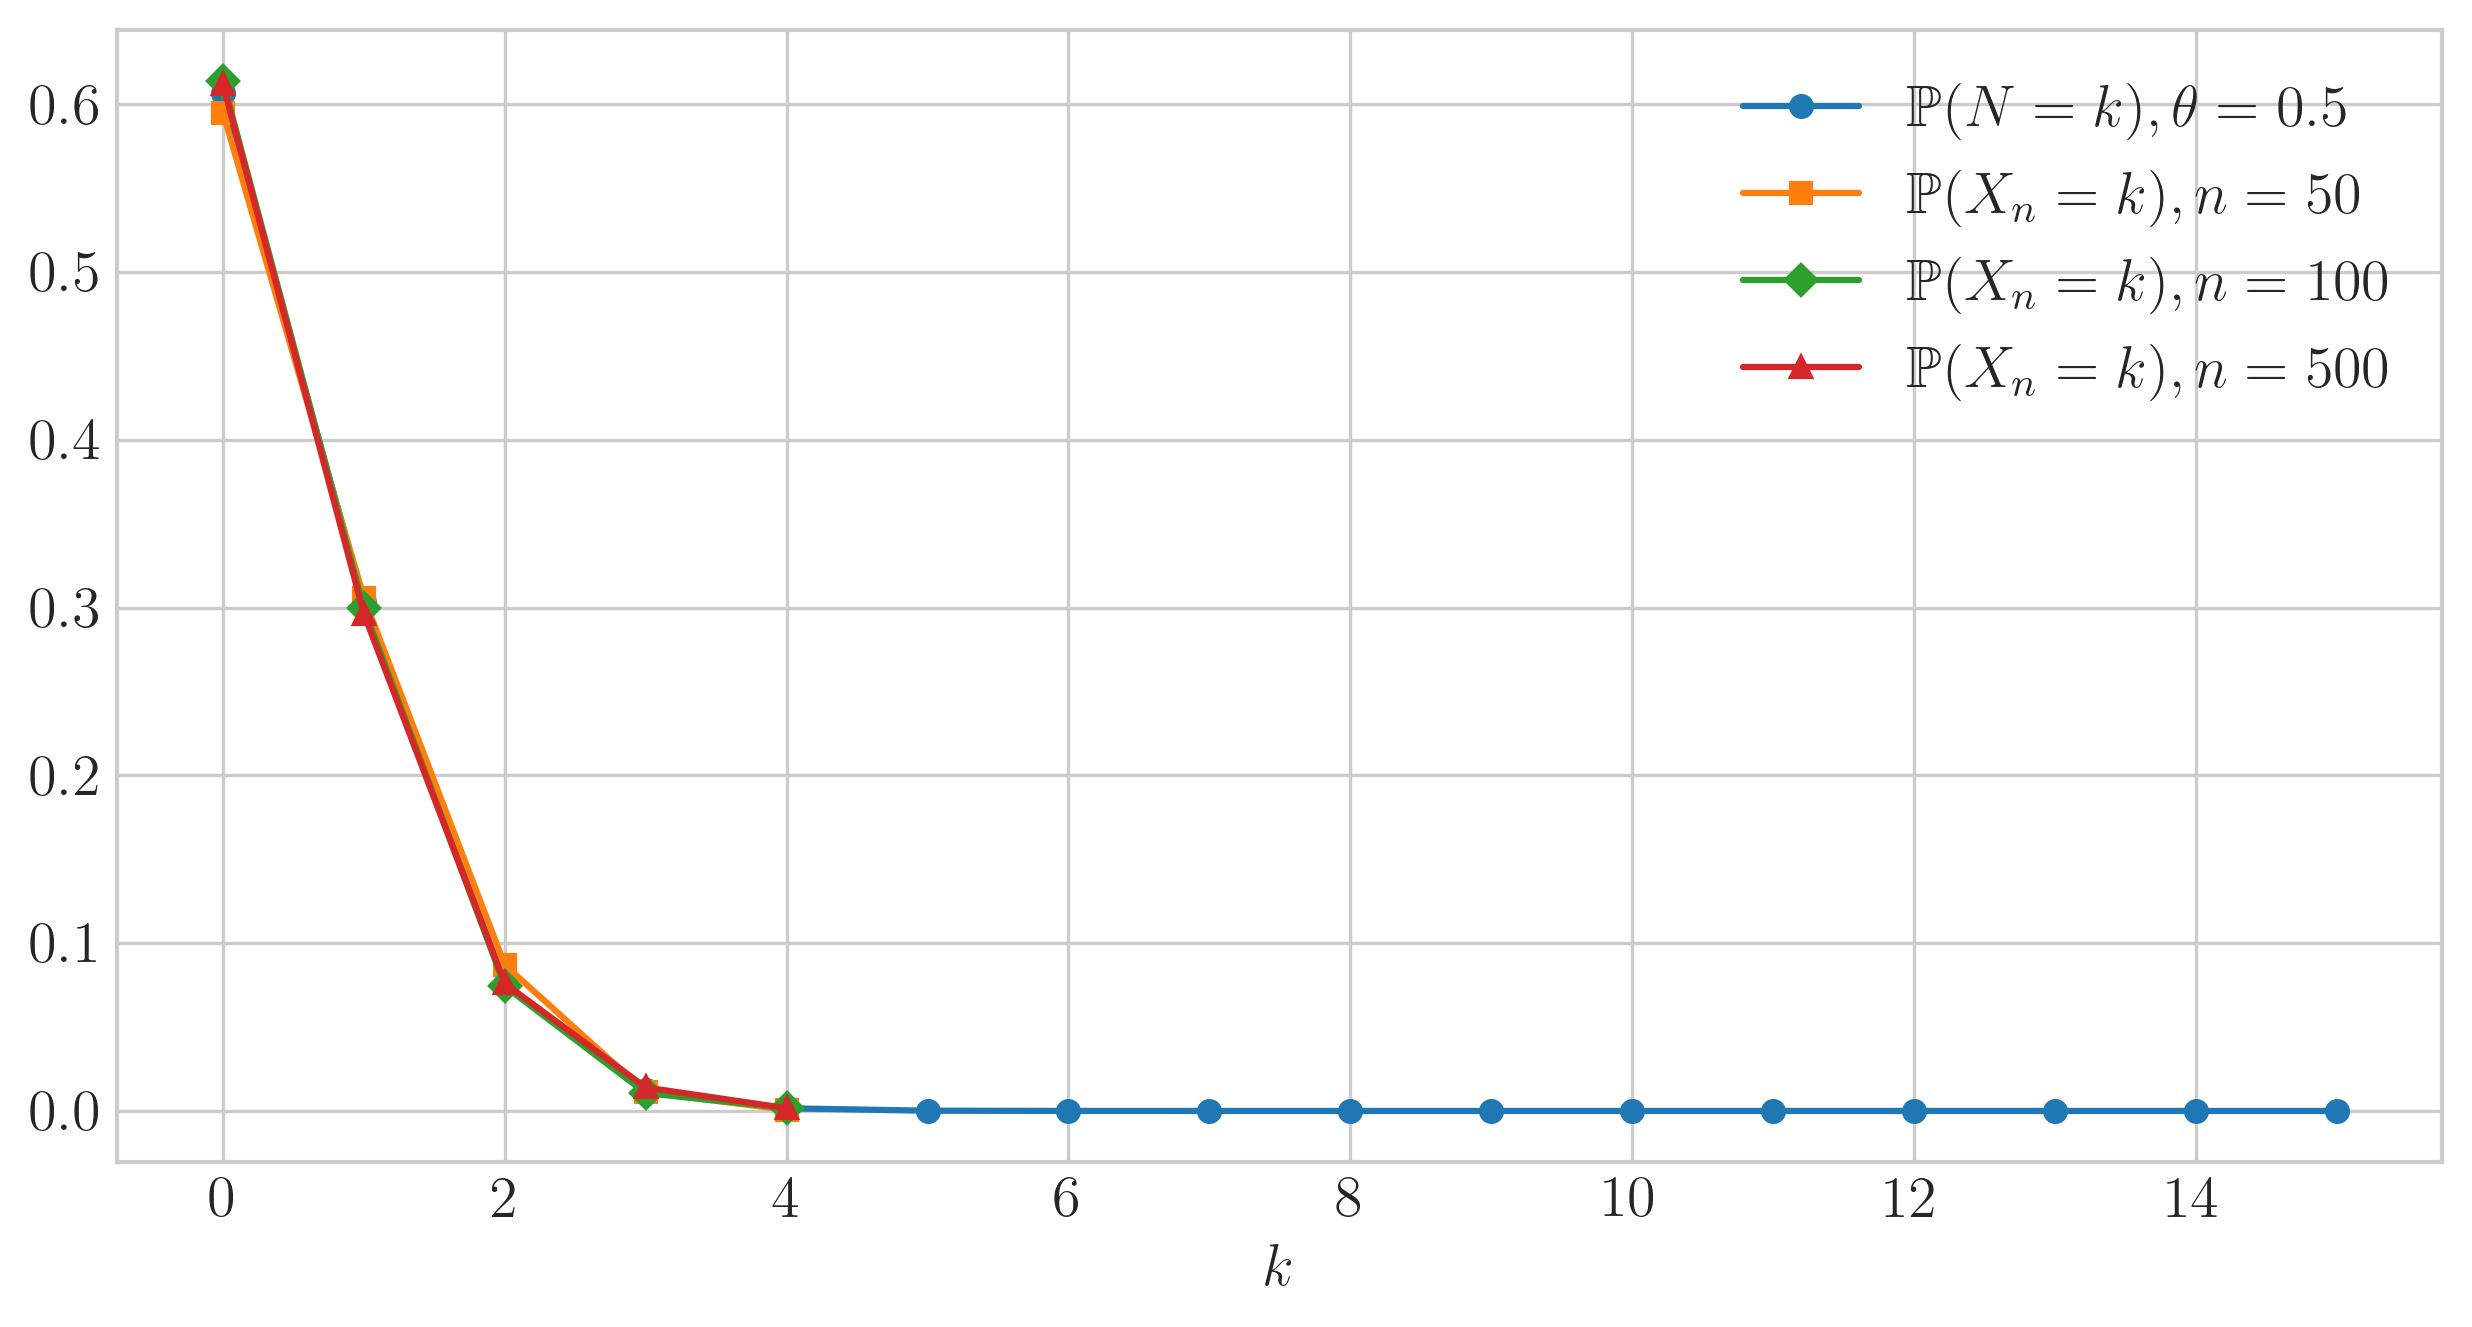
\includegraphics[scale=0.6]{plots/fp_prob_theta_0.5.png}
    \caption{Полігони розподілу $X_n$ та $N$ для $\theta = 0.5$.}
\end{figure}

\begin{figure}[H]
    \centering
    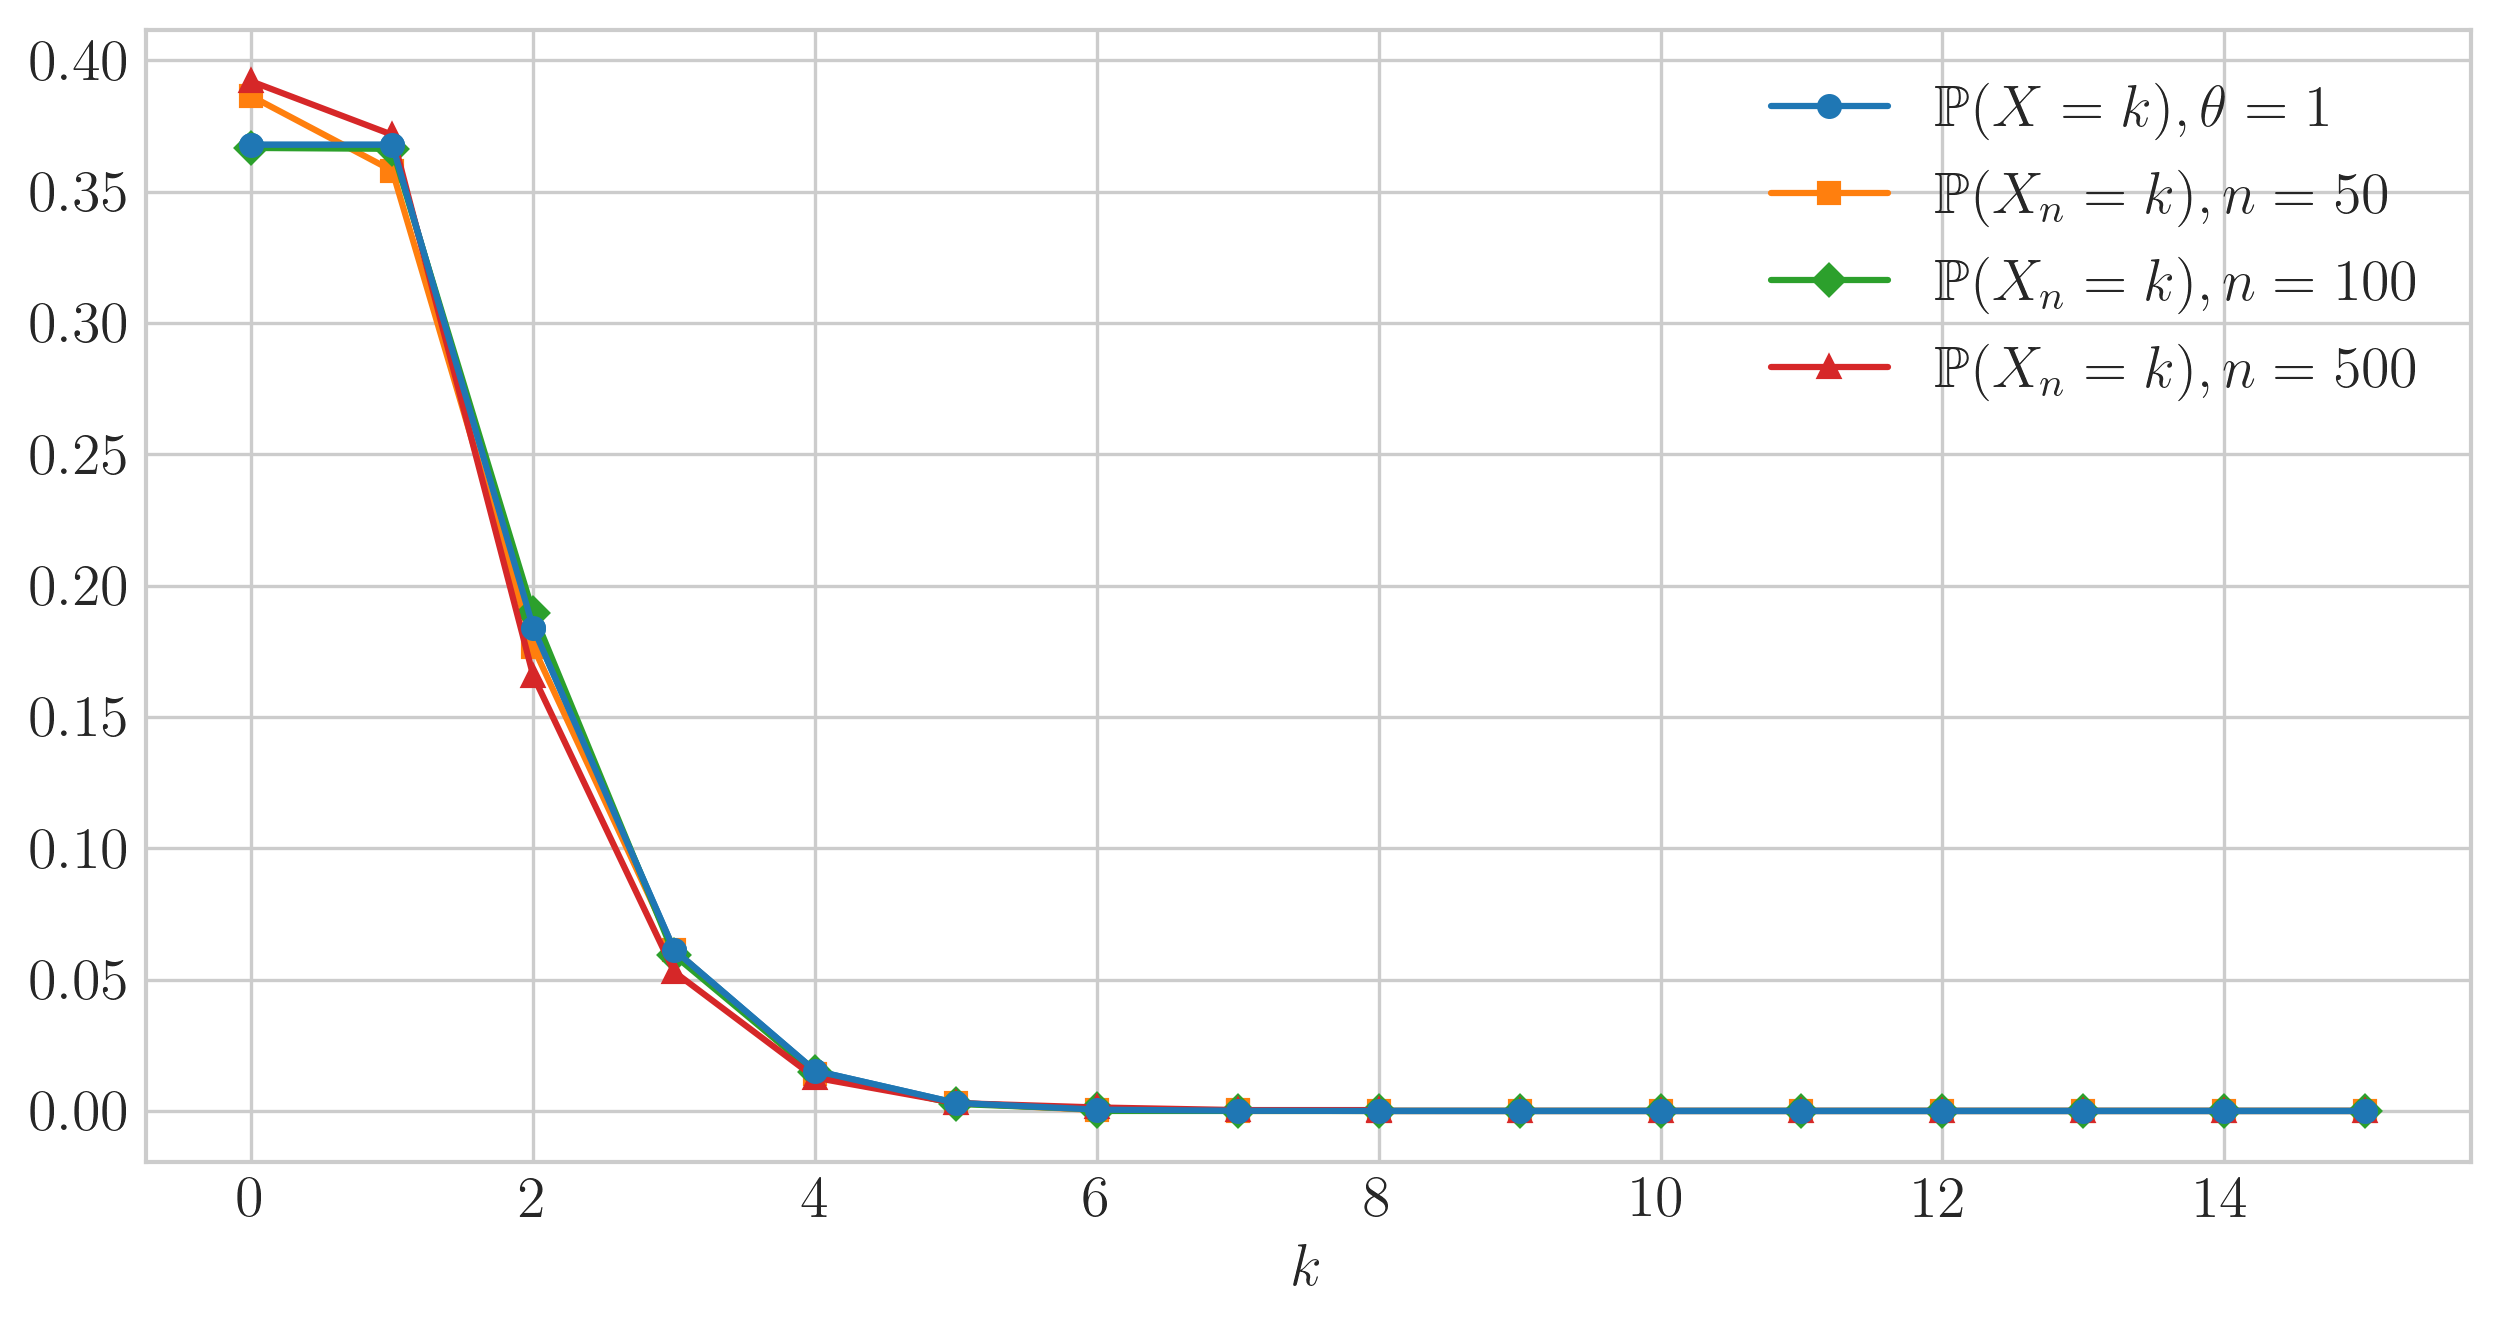
\includegraphics[scale=0.6]{plots/fp_prob_theta_1.png}
    \caption{Полігони розподілу $X_n$ та $N$ для $\theta = 1$.}
\end{figure}

\begin{figure}[H]
    \centering
    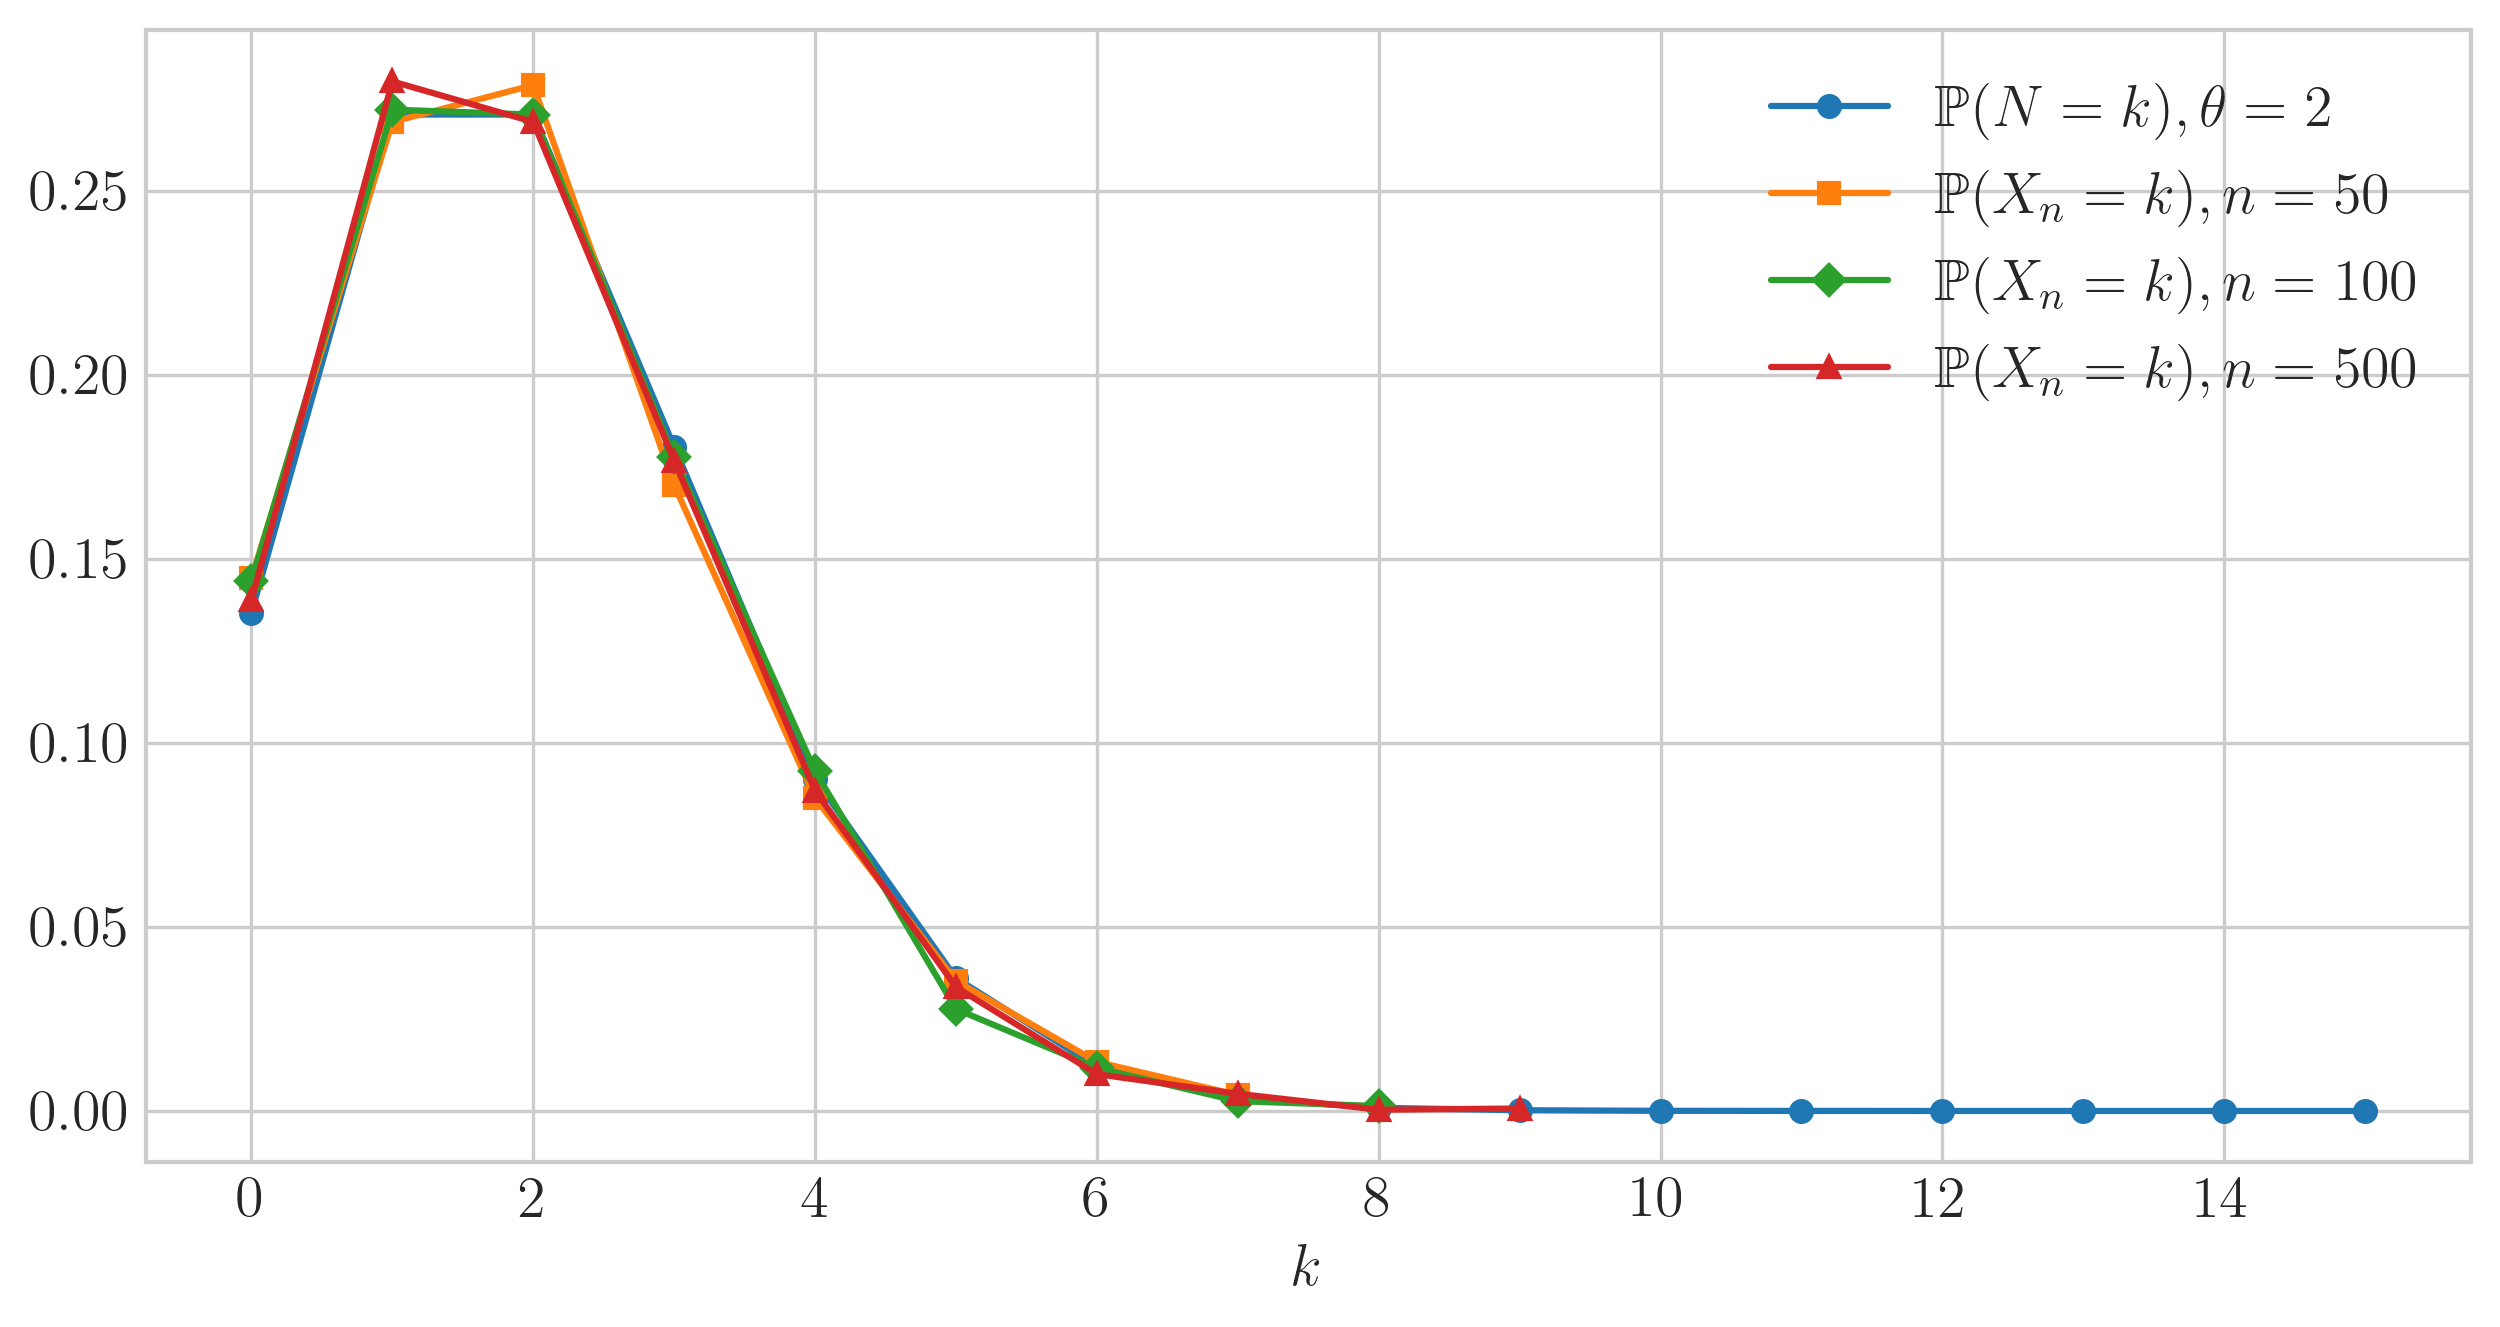
\includegraphics[scale=0.6]{plots/fp_prob_theta_2.png}
    \caption{Полігони розподілу $X_n$ та $N$ для $\theta = 2$.}
\end{figure}

\begin{figure}[H]
    \centering
    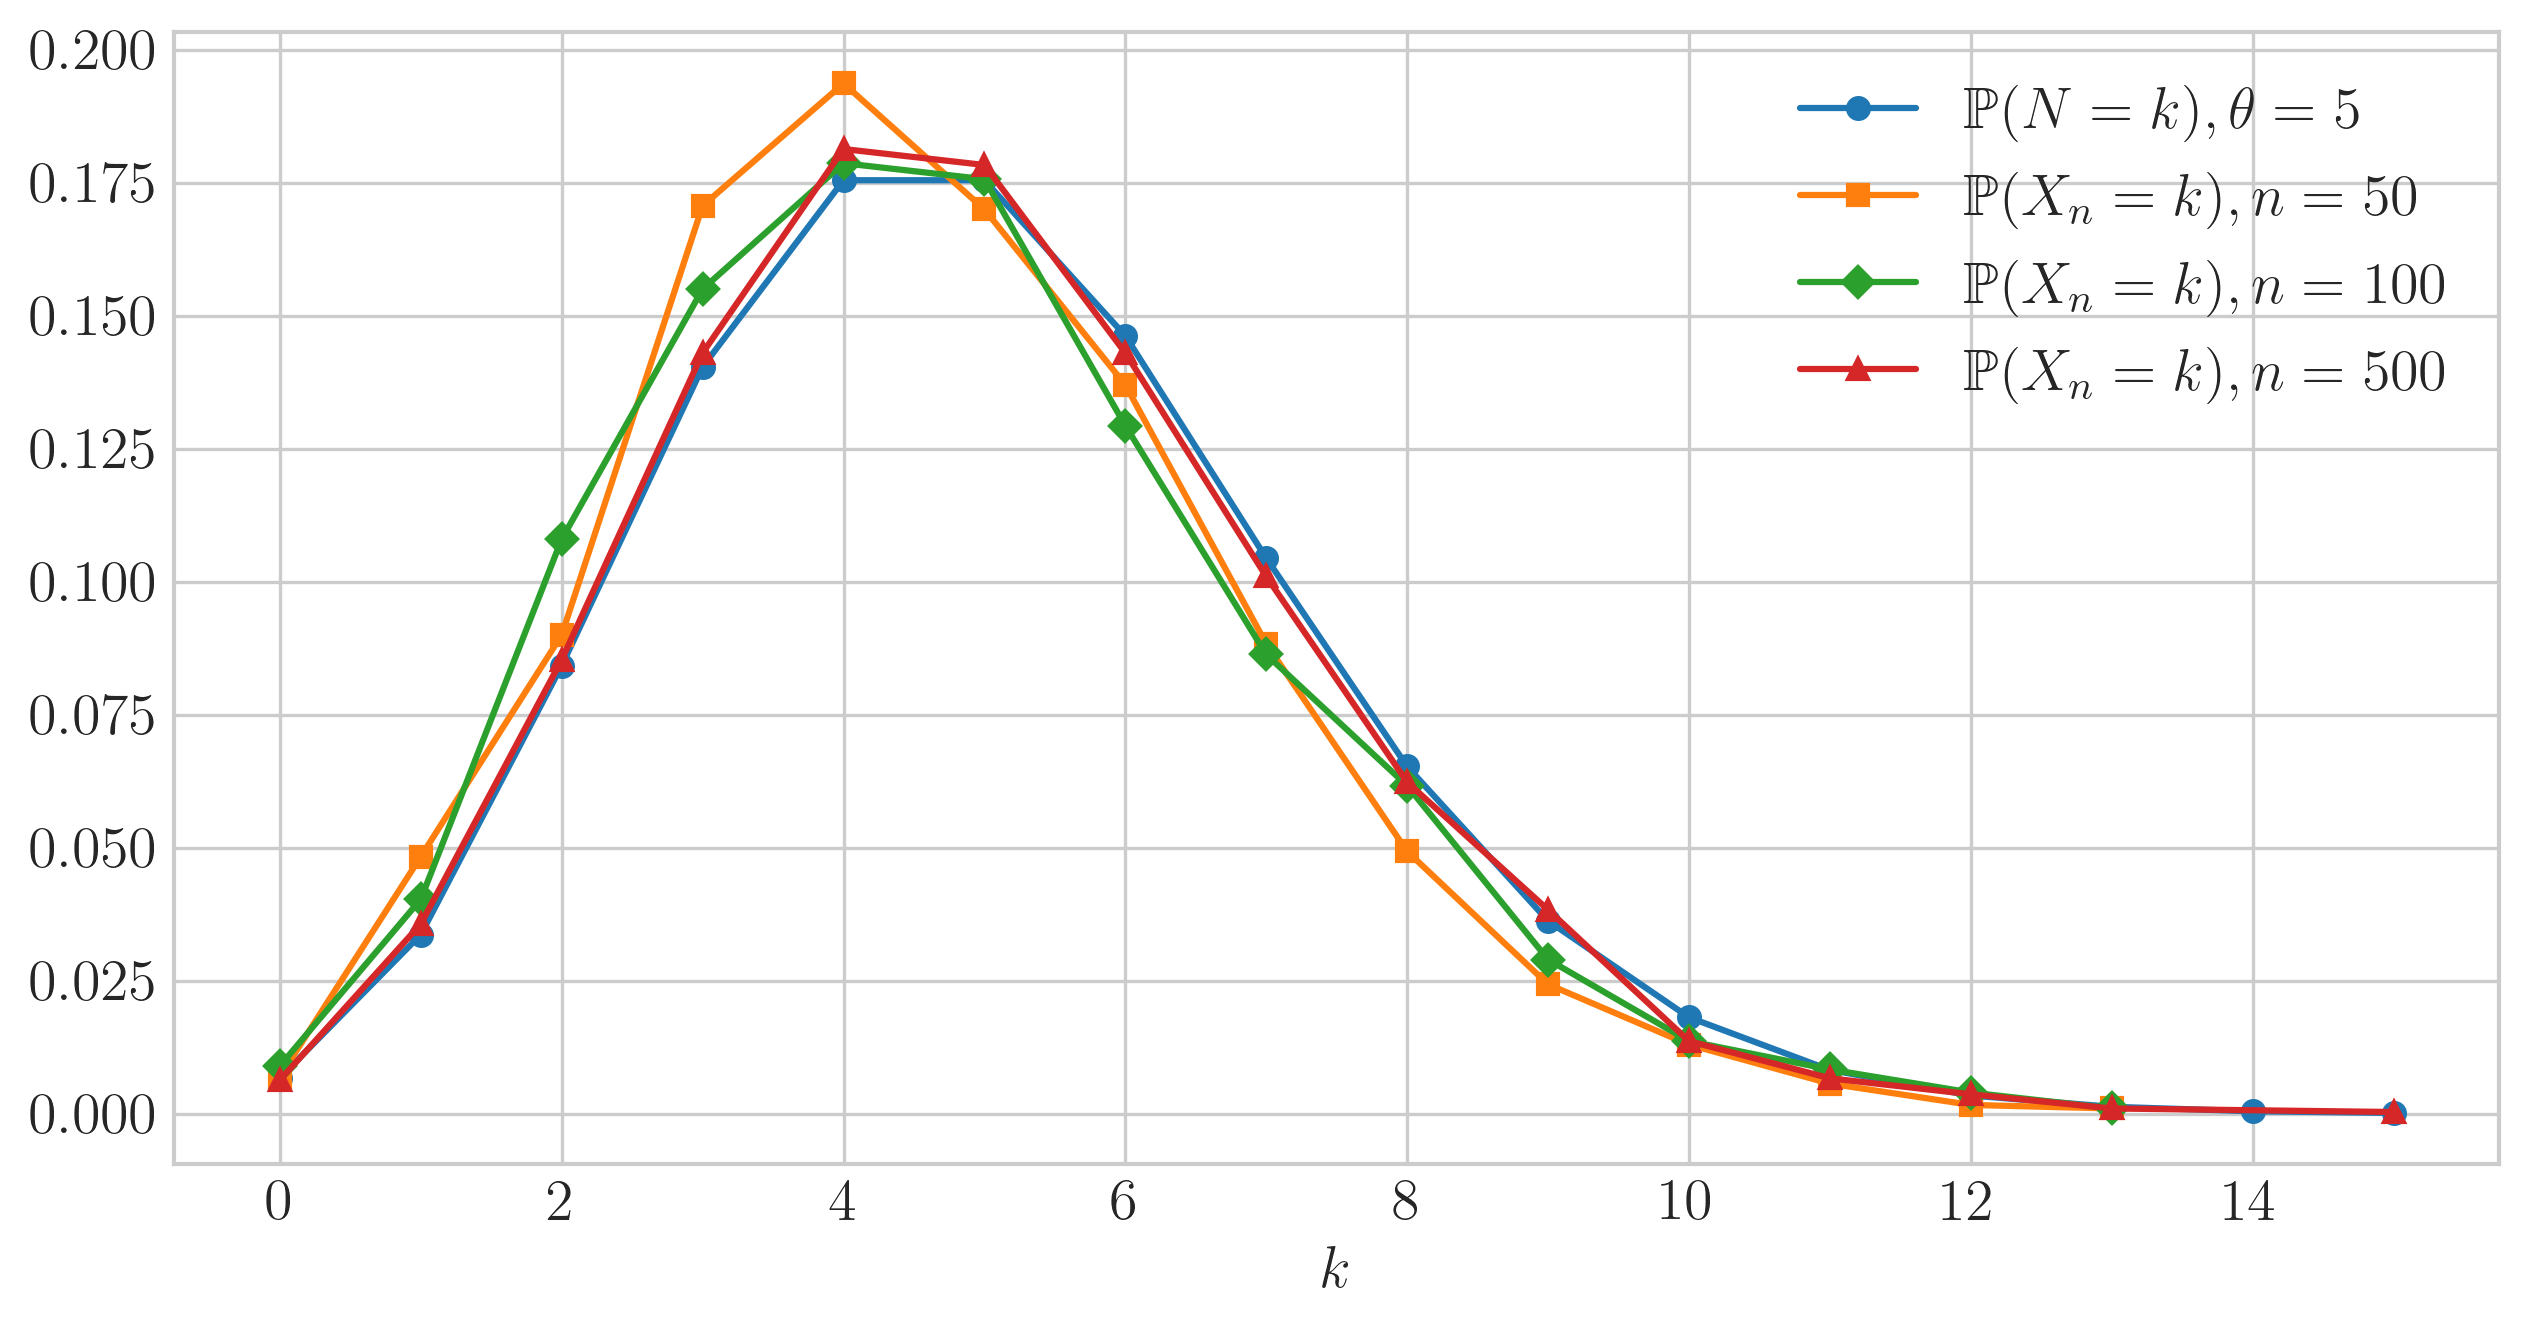
\includegraphics[scale=0.6]{plots/fp_prob_theta_5.png}
    \caption{Полігони розподілу $X_n$ та $N$ для $\theta = 5$.}
\end{figure}

Видно, що збіжність ймовірностей дійсно присутня, але для більших
значень $\theta$ вона є повільнішою.